\chapter{General Approach to the Problem}
\label{cha:approachestotheproblem}

In this chapter, our approach to find and repair conflicting spots in the netlists is described.

\section{Routing Elements in RapidSmith}
\label{sec:routingelementsinrapidsmith}

Since the RapidSmith API define multiple elements involved in the routing process, a short overview over these elements is given in the following list:
\begin{itemize}
\item \textbf{Wire}\hfill \\
A Wire is the basic connection element. It is represented as an integer due to the large number of wires on an FPGA. Wires can be hard connected to other wires, which can be determined through the \texttt{Device} class.
\item \textbf{Pin}\hfill \\
A Pin connects an input or output of a logic block to routing resources. It is primarily connected to one \texttt{wire}, and may be defined as output or input pin.
\item \textbf{PIP}\hfill \\
A PIP object describes an active connection between two wires, which are attributes to the object. If it is contained in a \texttt{net}, is is switched on. Otherwise, it remains turned off.
\item \textbf{Net}\hfill \\
A Net gathers a list of connected pins and active PIPs. It also has a defined source pin driving the net.
\item \textbf{WireConnection}\hfill \\
A WireConnection is a wrapper class for a \texttt{wire} and holds the information whether this wire is only reacheable if a PIP is turned on. This class is used to get information about the connectable wires on the FPGA.
\item \textbf{Node}\hfill \\
A Node is a routing object used in the router package. It can be used to describe routes of \texttt{wires} and \texttt{PIPs} in a router.
\item \textbf{SinkPin}\hfill \\
A SinkPin refers to a switch matrix on the FPGA. Nearly all pins' wires are connected to a switch matrix, which is an interface to the other wires. SinkPins have to be viewed if a connected pin of a wire shall be found.
\item \textbf{Tile}\hfill \\
A Tile is one of the checkerboard-like distributed areas on an FPGA. It holds various elements from the list above and a set of logic elements. 

\end{itemize}

\section{Isoelectric Potential Search}
\label{sec:isolectricelements}

Each design's routing in RapidSmith can be viewed as a set of \texttt{Net} objects. According to the RapidSmith documentation \cite{rapidsmith}, these \texttt{Net} objects hold all used pins and pips of the net.
Therefore it should be possible to reach all sink pins of a net by following wires connected to the input pin if the net is not broken.
Consequently each design is broken if it is not possible to reach the output pins of an net from the input pin.  

A \texttt{Net} in RapidSmith only contains \texttt{PIP} objects representing PIPs that are currently "switched on", but no \texttt{Wires}. Therefore, a net can be expanded if additional PIPs are switched on. 
It is theorized that it is possible to fix the broken net by switching on PIPs which reconnect the net's pins' connected wires with each other. This can only be done when the PIP will not connect the circuit to an independent third circuit.

To check whether or not a net can be traversed from it's source pin to all output pins an new measurement called \texttt{Potential} is introduced into RapidSmith.
A \texttt{Potential} can be seen as the isoelectric set of wires, pins and PIPs which are connected, starting from one pin.
It is never possible for a \texttt{Pin}, \texttt{PIP} or \texttt{Wire} to be in two \texttt{Potential}s at the same time. It is not possible that two non-connected elements have the same \texttt{Potential}. 
This concept is named after the concept of isoelectric potentials found in classical electronics. Although two electrical potentials may be at the same numeric voltage level and still be different (not isoelectric), this is not the case for the introduced potentials.

Before any further operation on a \texttt{Potential} may be performed, its spatial spread must be computed. This means that, starting from a pin, each electrically connected wire, pin and pip must be found. The search for connected elements works as described in algorithm \ref{alg:findingpotential}. It is also pointed graphically in Figure \ref{fig:buildpotential}. Given this method, a \texttt{Potential} derived for one pin must always hold any other pin in the net if the net is routed correctly.

\begin{algorithm}[h]
	wires = \{wireOf(sourcePin)\};\\
	pips = \{\};\\
	pins = \{sourcePin\};\\
	adjacentPIPs = \{\};\\
	\While{new elements added}{
	\ForEach{wire i}{
	  \ForEach{reacheableWire(i)}{
			\If{!reacheable.isPIP()}{
				add reacheableWire to wires;\\
			}{
				\ElseIf{pip $\in$ net.pips()}{
					add reacheableWire to wires;\\
					add pip to pips;\\
				}
				\Else{
					add pip to adjacentPIPs;\\
					}
			}
	   	}
	  }
	}	
	\ForEach{wire i}{
		add connected pin to pins;\\
	}
 \caption{Algorithm to determine all elements on one isoelectric potential.}
 \label{alg:findingpotential}
\end{algorithm}

\begin{figure}
\centering
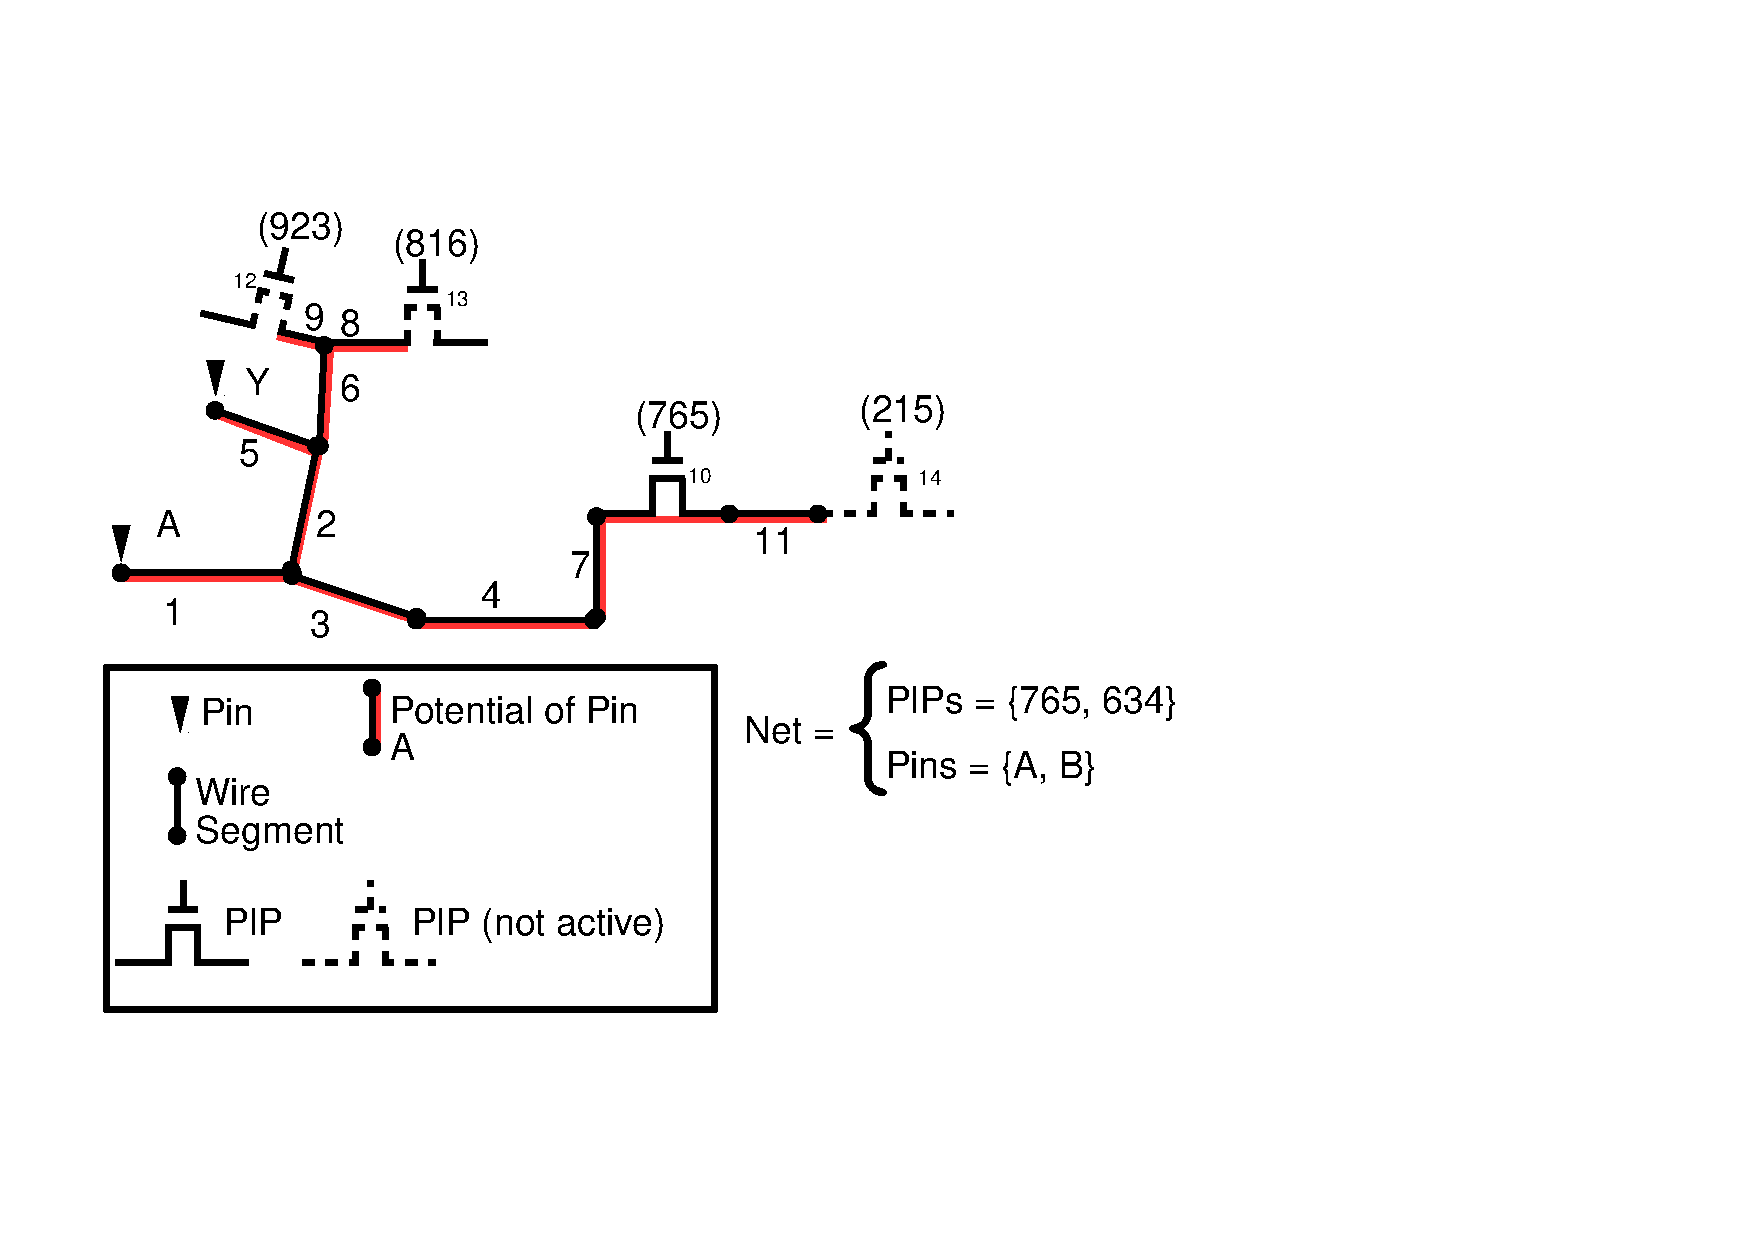
\includegraphics[scale=0.8]{images/buildpotential_buildup.pdf}
\caption{Graphical visualization of the \texttt{Potential} derivation. The wire segments and elements are enumerated in the sequence of integration. PIP IDs are in parentheses.}
\label{fig:buildpotential}
\end{figure}



\texttt{Potential}s can be fused by setting PIPs. Electrically, this means that two isoelectric sets of elements are connected by a switch, and thus become one isoelectric potential. For the object representation this means that, if a PIP is set, the two \texttt{Potential} objects have to be united.

In order to keep track of the switchable conenctions to other potentials, each potential has a set of adjacent \texttt{PIP}s. When the potential is created and its spread is computed, every \texttt{PIP} which is connected to any wire of the potential, but not specified to be switched on by the net, is added to the adjacent PIP set. Hence, all PIPs which can be reached from the pins in the \texttt{Potential} are stored.

The concept of isoelectric potentials is chosen because the search for adjacent pips wire by wire is simplified this way.


\newpage
\section{Finding and Reparing broken Nets}
\label{sec:findingandrepairingbrokennets}

In order to check if an net is broken the potential of each pin is calculated and compared. If the net contains more than one unique potential then the net is broken.
In that case it is necessary to reconnect the two parts (potentials) of that net. If the assumption that only one or two PIPs are missing is true, this can be done by the applying the following breadth-first-search on the \texttt{Potential}s of pins A and B:

\begin{algorithm}[H]
	add all adjacent PIPs of A to leaves;\\
	\While{leaves.size() > 0}{
		PIP pip = leaves.pop(); \\
		\If{Potential B contains pip}{
			return pip; // we can determine the connection trough the parent PIPs;\\
		}
		\ForEach{PIP p $\in$  adjacentPIPs(potential of pip)}{
			\If{p!=pip.parent}{
				leaves.push(p); //if p is of an other potential than B we cannot add it ;\\
				}
		}
	}
 \caption{Exemplary algorithm to determine missing PIPs by breadth-first-search}
 \label{alg:breadth-first-search}
\end{algorithm}


There is a priority queue \textit{leaves} which holds only PIP-elements that do not connect to other \texttt{Potential}s besides B. 
Each of these elements has a parent PIP which introduced the PIP into the queue. \textit{Leaves} is ordered by the number of parents between the PIP and Potential A in ascending order. Algorithm \ref{alg:breadth-first-search} points out the search on that priority queue.



Figure \ref{fig:brokenpotentials} shows the case for one non-set PIP in a net. The net specifies two pins, A and B. For both pins, the \texttt{Potential} has been determined. Clearly marked are the included wires, PIPs and other pins. PIP 215 is adjacent to both potentials. The breadth-first-search finds PIP 215 to be adjacent to both pins' potentials, so this PIP has to be set (a \texttt{PIP} instance is created for the connected \texttt{wires} and added to the net). For situations where more than one PIP has to be set, the breadth-first-search steps one level down the search tree and repeats the search on every leaf. By going one level deeper, the first PIP in the priority queue has to be set.

As one can see, the breadth-first search runtime highly depends on the number of missing PIPs in the net. For every missing PIP, the number of elements to search is multiplied by the amount of adjacent PIPs to the Potential.

\begin{figure}[h]
\centering
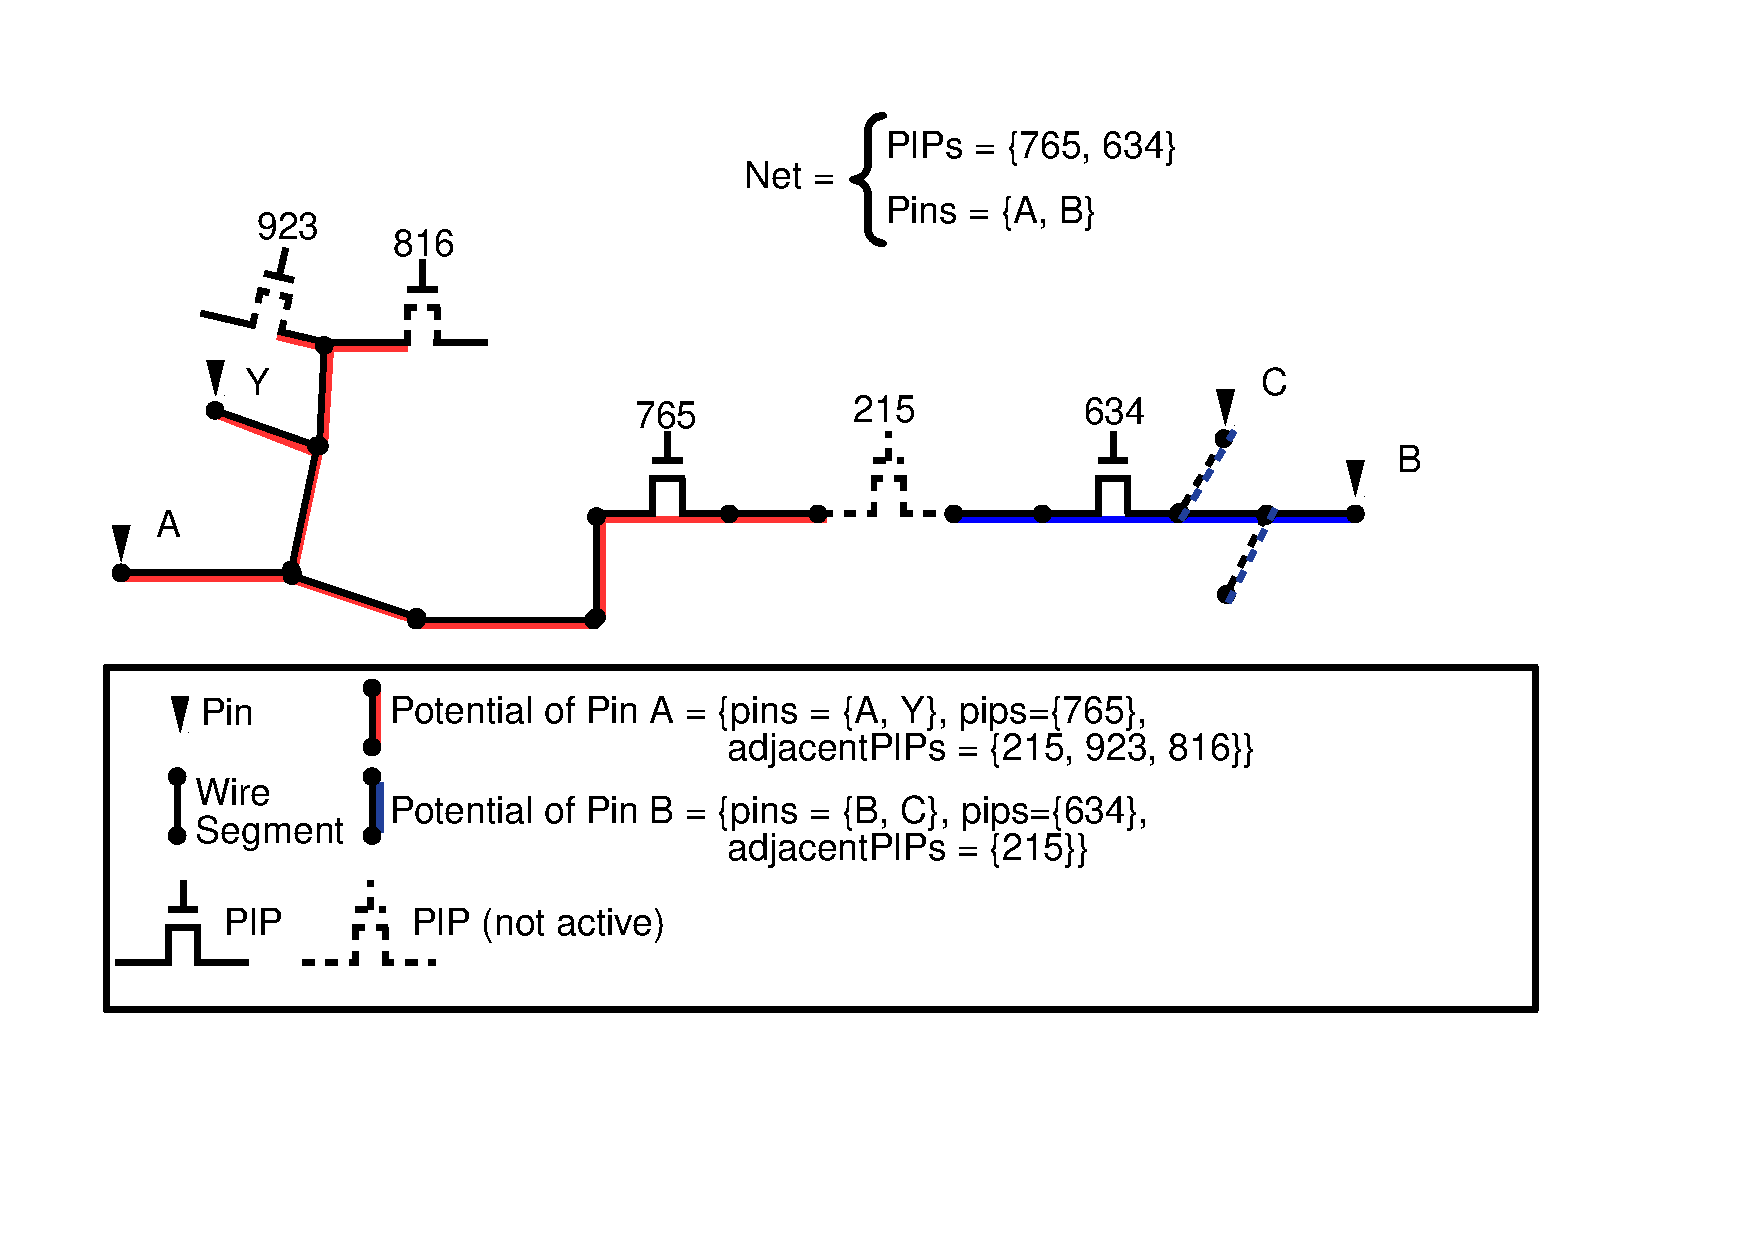
\includegraphics[scale=0.65]{images/brokenpotentials.pdf}
\caption{A net with two \texttt{Potentials} which have to be connected.}
\label{fig:brokenpotentials}
\end{figure}



